\subsection{O ambiente}
O ambiente consiste em uma espaço de 100$m^2$ delimitado por paredes e diversos ``postes'' de formato cilíndrico de 16$cm$ de diâmetro, e está representado na Figura \ref{fig:environment}.
\begin{figure}[h]
  \begin{subfigure}{.50\textwidth}
    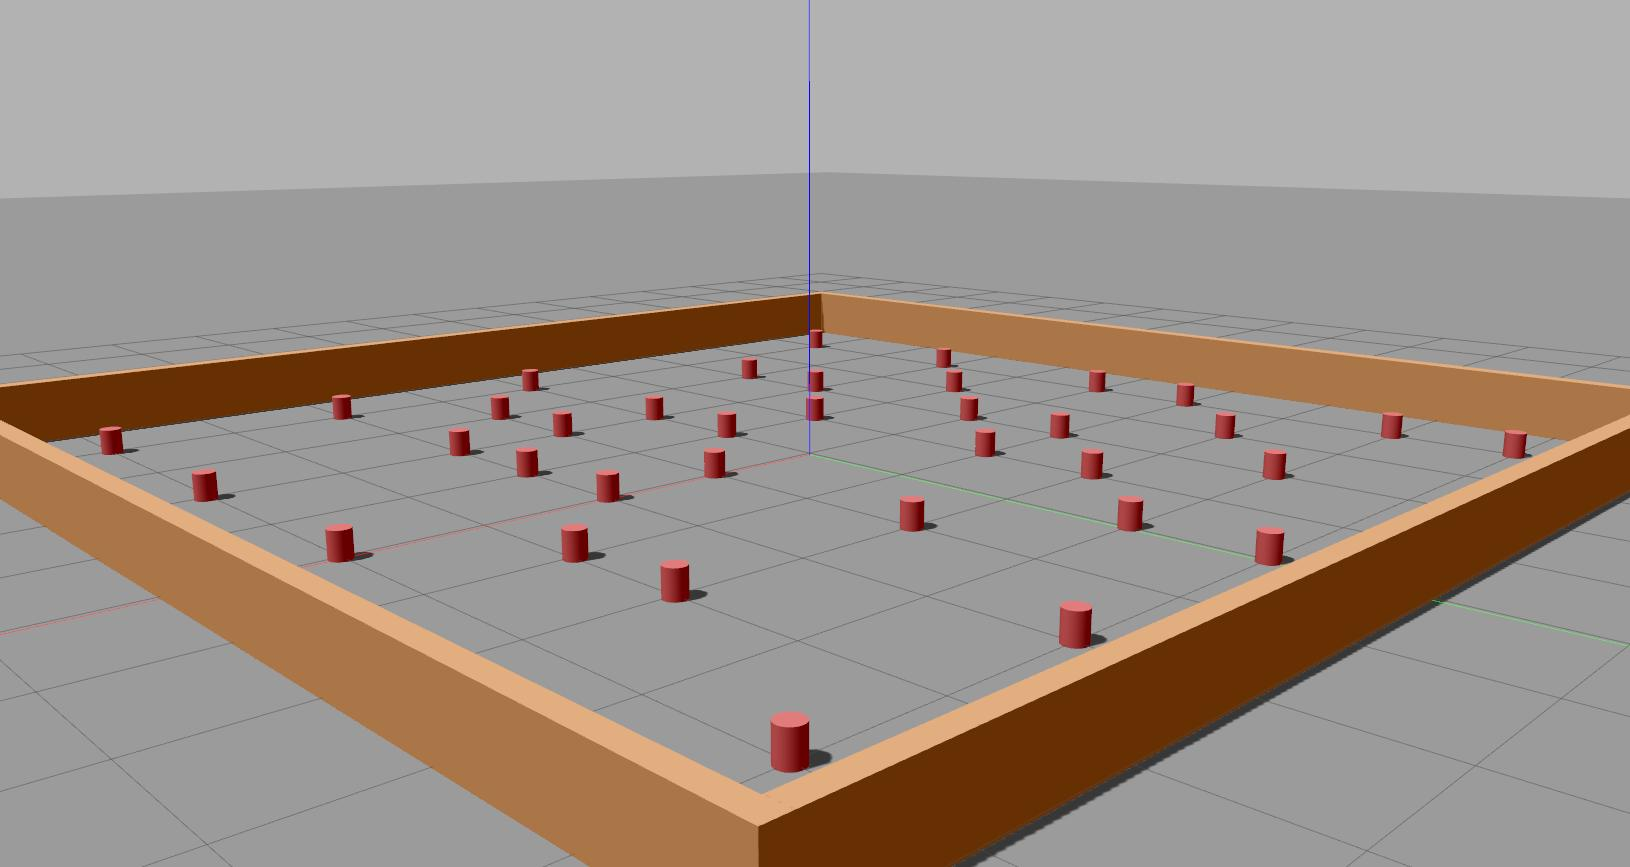
\includegraphics[width=\textwidth]{figs/environment-perspective.jpg}
    \caption{Vista perspectiva ampla}
  \end{subfigure}
  \hfill
  \begin{subfigure}{.50\textwidth}
    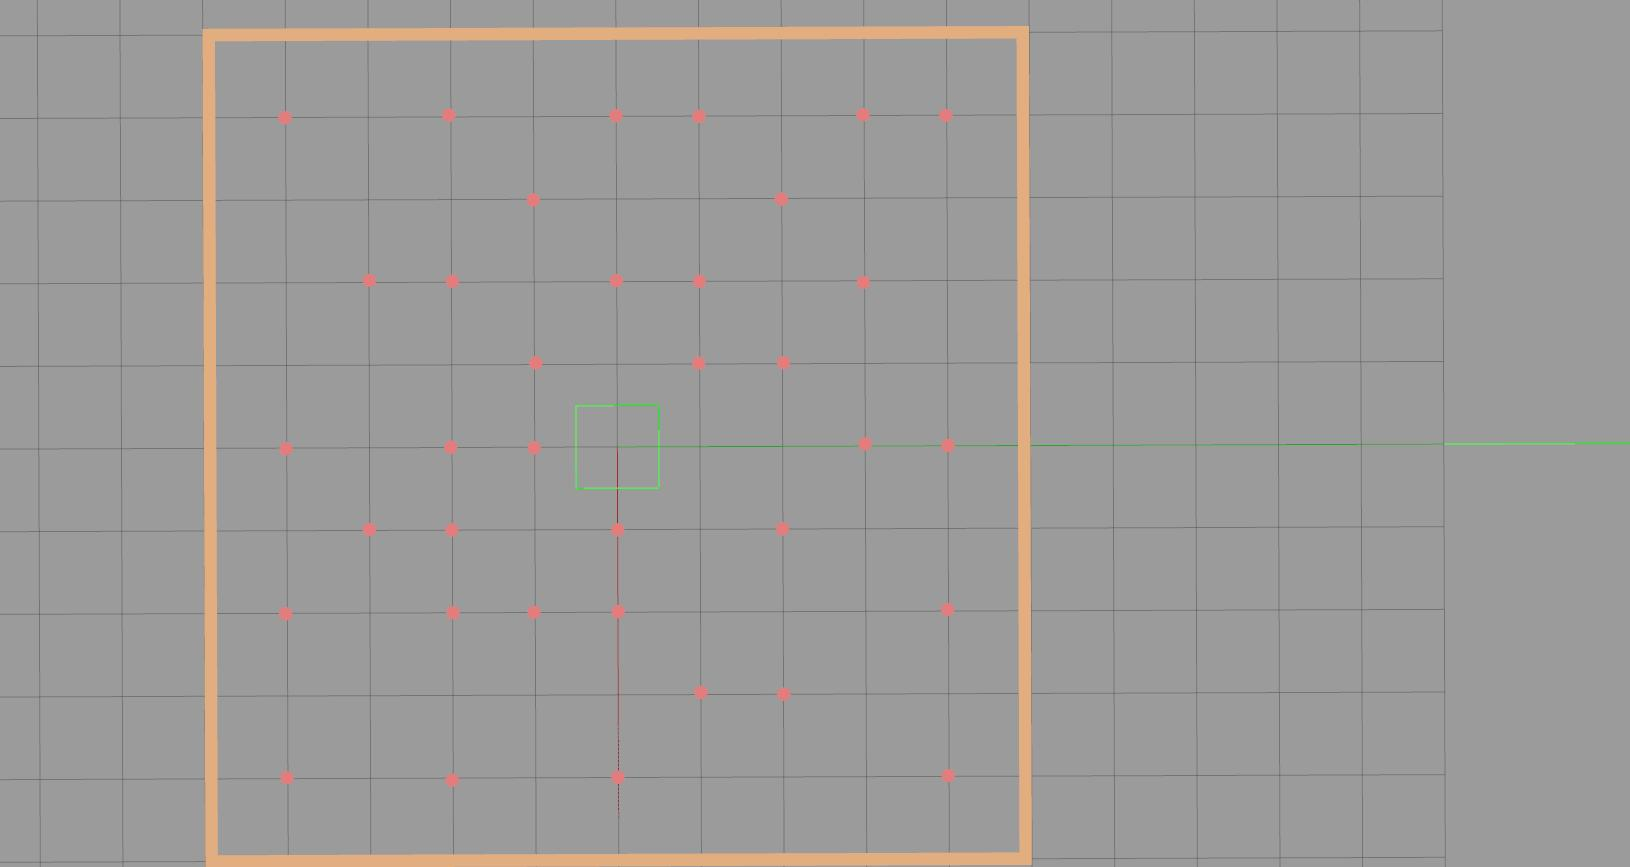
\includegraphics[width=\textwidth]{figs/environment-birds-eye-of-view.jpg}
    \caption{Vista ortográfica superior}
  \end{subfigure}
  \hfill
  \begin{subfigure}{\textwidth}
    \centering
    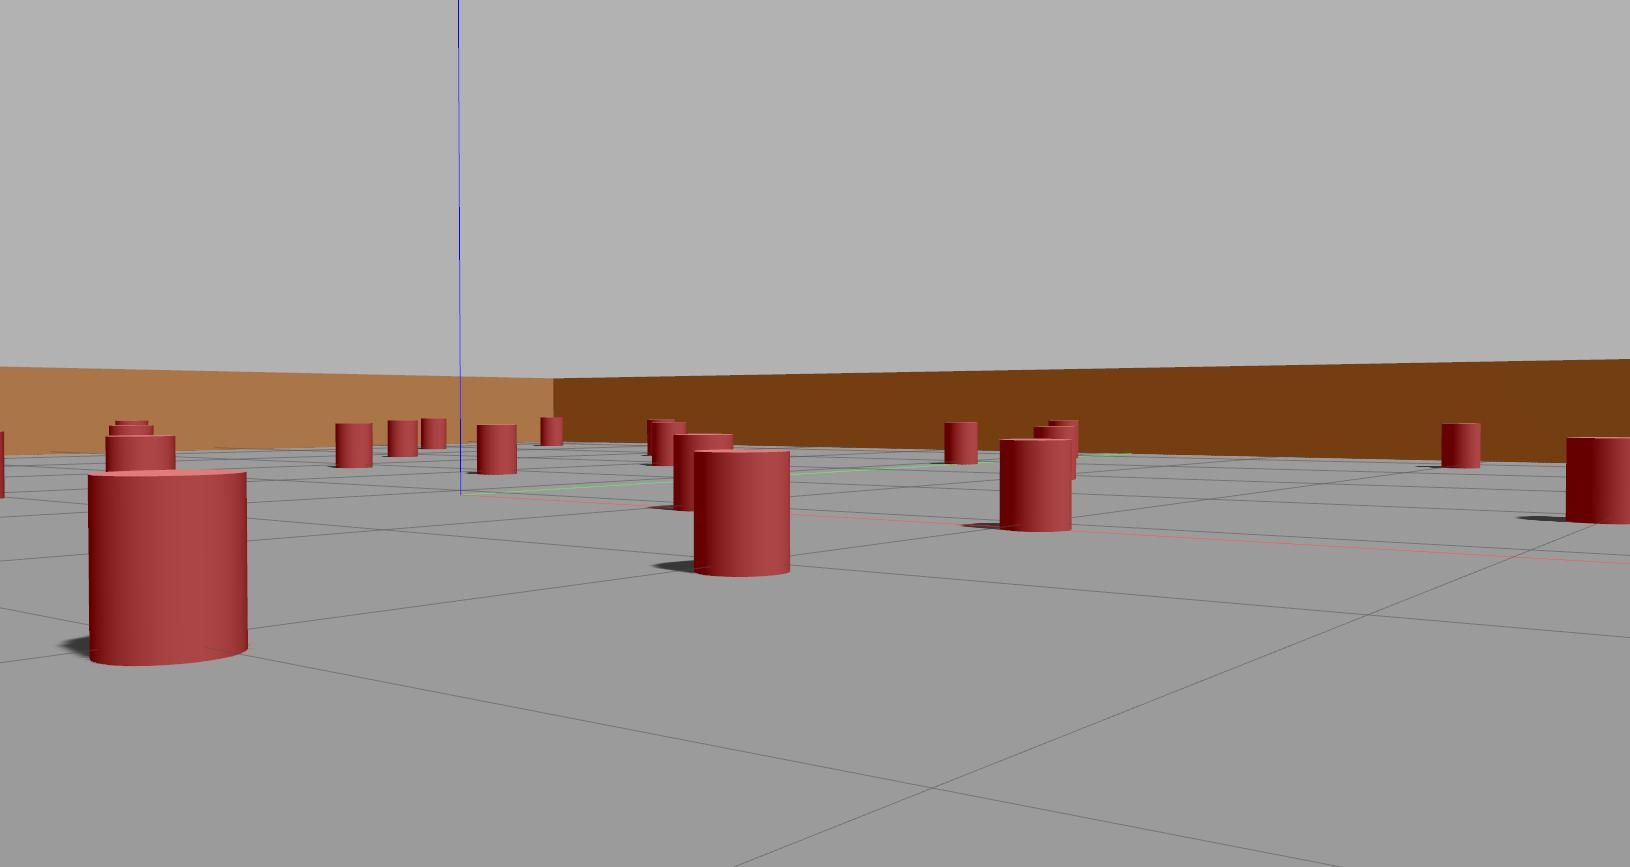
\includegraphics[width=.5\textwidth]{figs/environment-closer-perspective.jpg}
    \caption{Vista perspectiva fechada}
  \end{subfigure}
  \caption{Diferentes vistas do ambiente simulado}
  \label{fig:environment}
\end{figure}

\subsection{O robô}
Neste trabalho foi utilizado o modelo do robô \emph{Turtlebot 3} \cite{TurtleBot_3} exibido na Figura \ref{fig:turtlebot-digital-twin}, que é um robô de acionamento diferencial equipado com 
\textit{encoder} de rodas, uma IMU e um sensor laser do tipo LiDAR.
\begin{figure}[h]
  \centering
  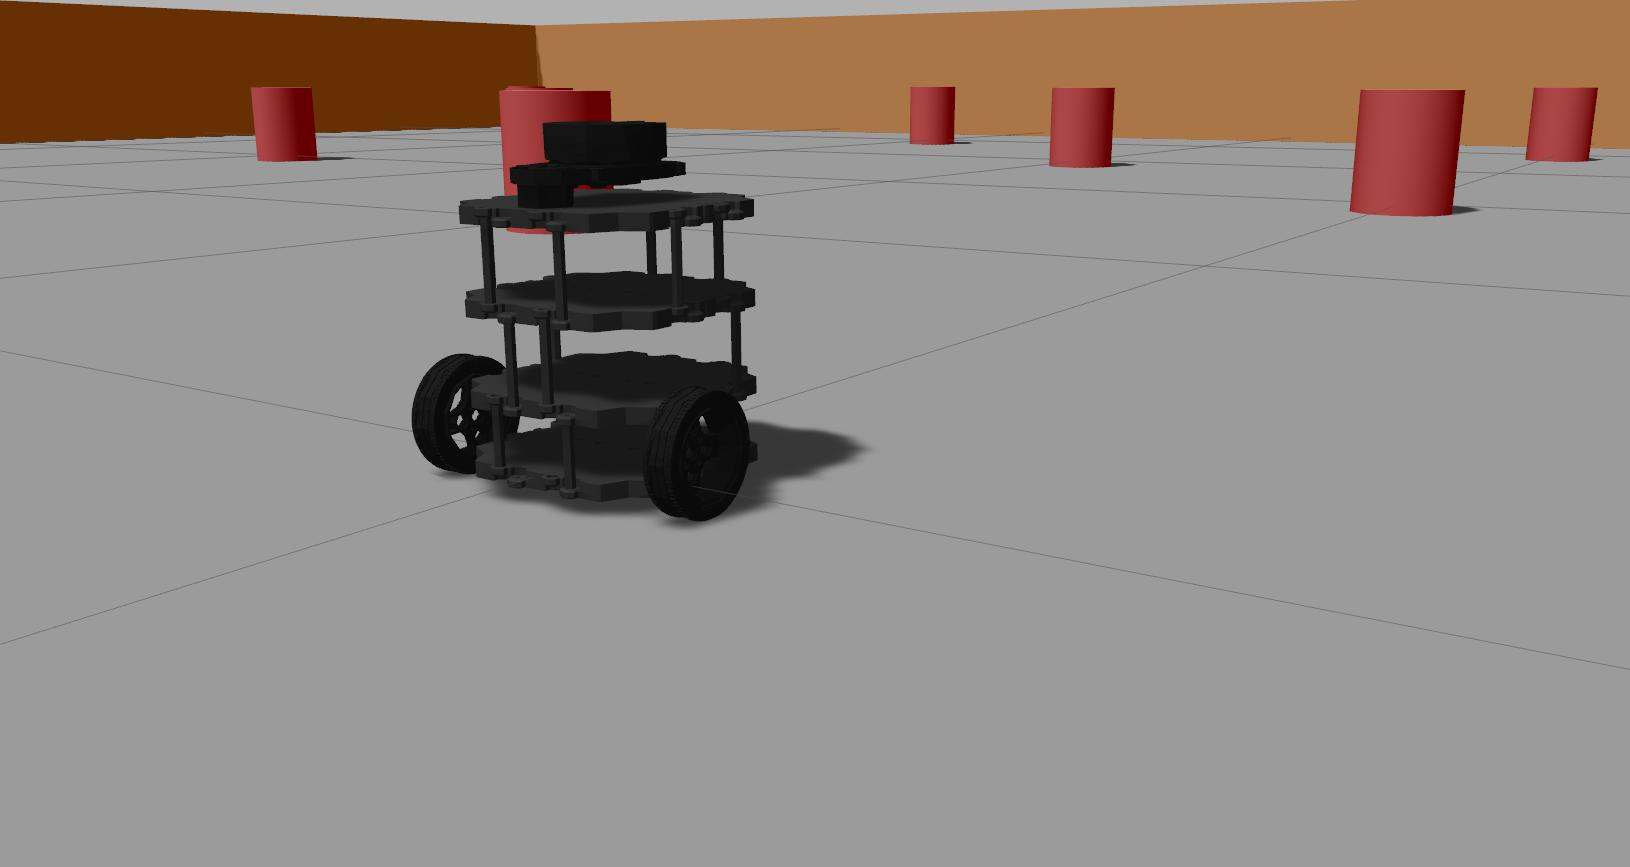
\includegraphics[width=0.7\textwidth]{figs/robot-closeup.jpg}
  \caption[Modelo do robô \textit{Turtlebot 3}]{Modelo do robô \textit{Turtlebot 3}. O sensor LiDAR encontra-se no topo do robô.}
  \label{fig:turtlebot-digital-twin}
\end{figure}